\section{Practical Recipe}
\label{sec:recipe}

In \Cref{sec:phenomenology}, we identified two conditions for successful OPD.
While possessing new knowledge is an intrinsic property of the teacher, the thinking-pattern gap between the teacher and the student can be narrowed through training design.
In this section, we present two complementary strategies that recover OPD in otherwise failing configurations by improving the overlap dynamics.

\begin{tcolorbox}[takeawaysbox]
\begin{itemize}[topsep=0pt, partopsep=0pt, leftmargin=12pt, itemsep=0pt]
  \item \textbf{Off-policy cold start (\Cref{sec:off_distill_matters}).} Fine-tuning the student on teacher-generated rollouts before OPD closes the initial thinking-pattern gap, leading to higher overlap from the start and consistently stronger final performance.
  \item \textbf{Teacher-aligned prompts (\Cref{sec:teacher_posttrain_data}).} Using prompts from the teacher's post-training data sharpens alignment on high-probability tokens, although such prompts should be mixed with out-of-distribution prompts to prevent entropy collapse.
\end{itemize}

\end{tcolorbox}

\subsection{Off-Policy Distillation from Teacher Rollouts as Cold Start}
\label{sec:off_distill_matters}

When the student and teacher have substantially different thinking patterns, pure OPD can be ineffective because the teacher's token-level supervision is difficult for the student to exploit from its initial policy.
To mitigate this mismatch, we consider a two-stage framework: we first perform off-policy distillation by supervised fine-tuning (SFT) the student on teacher-generated rollouts to bring it closer to the teacher's thinking pattern, and then continue training with standard OPD.

\begin{figure*}[t]
    \centering
    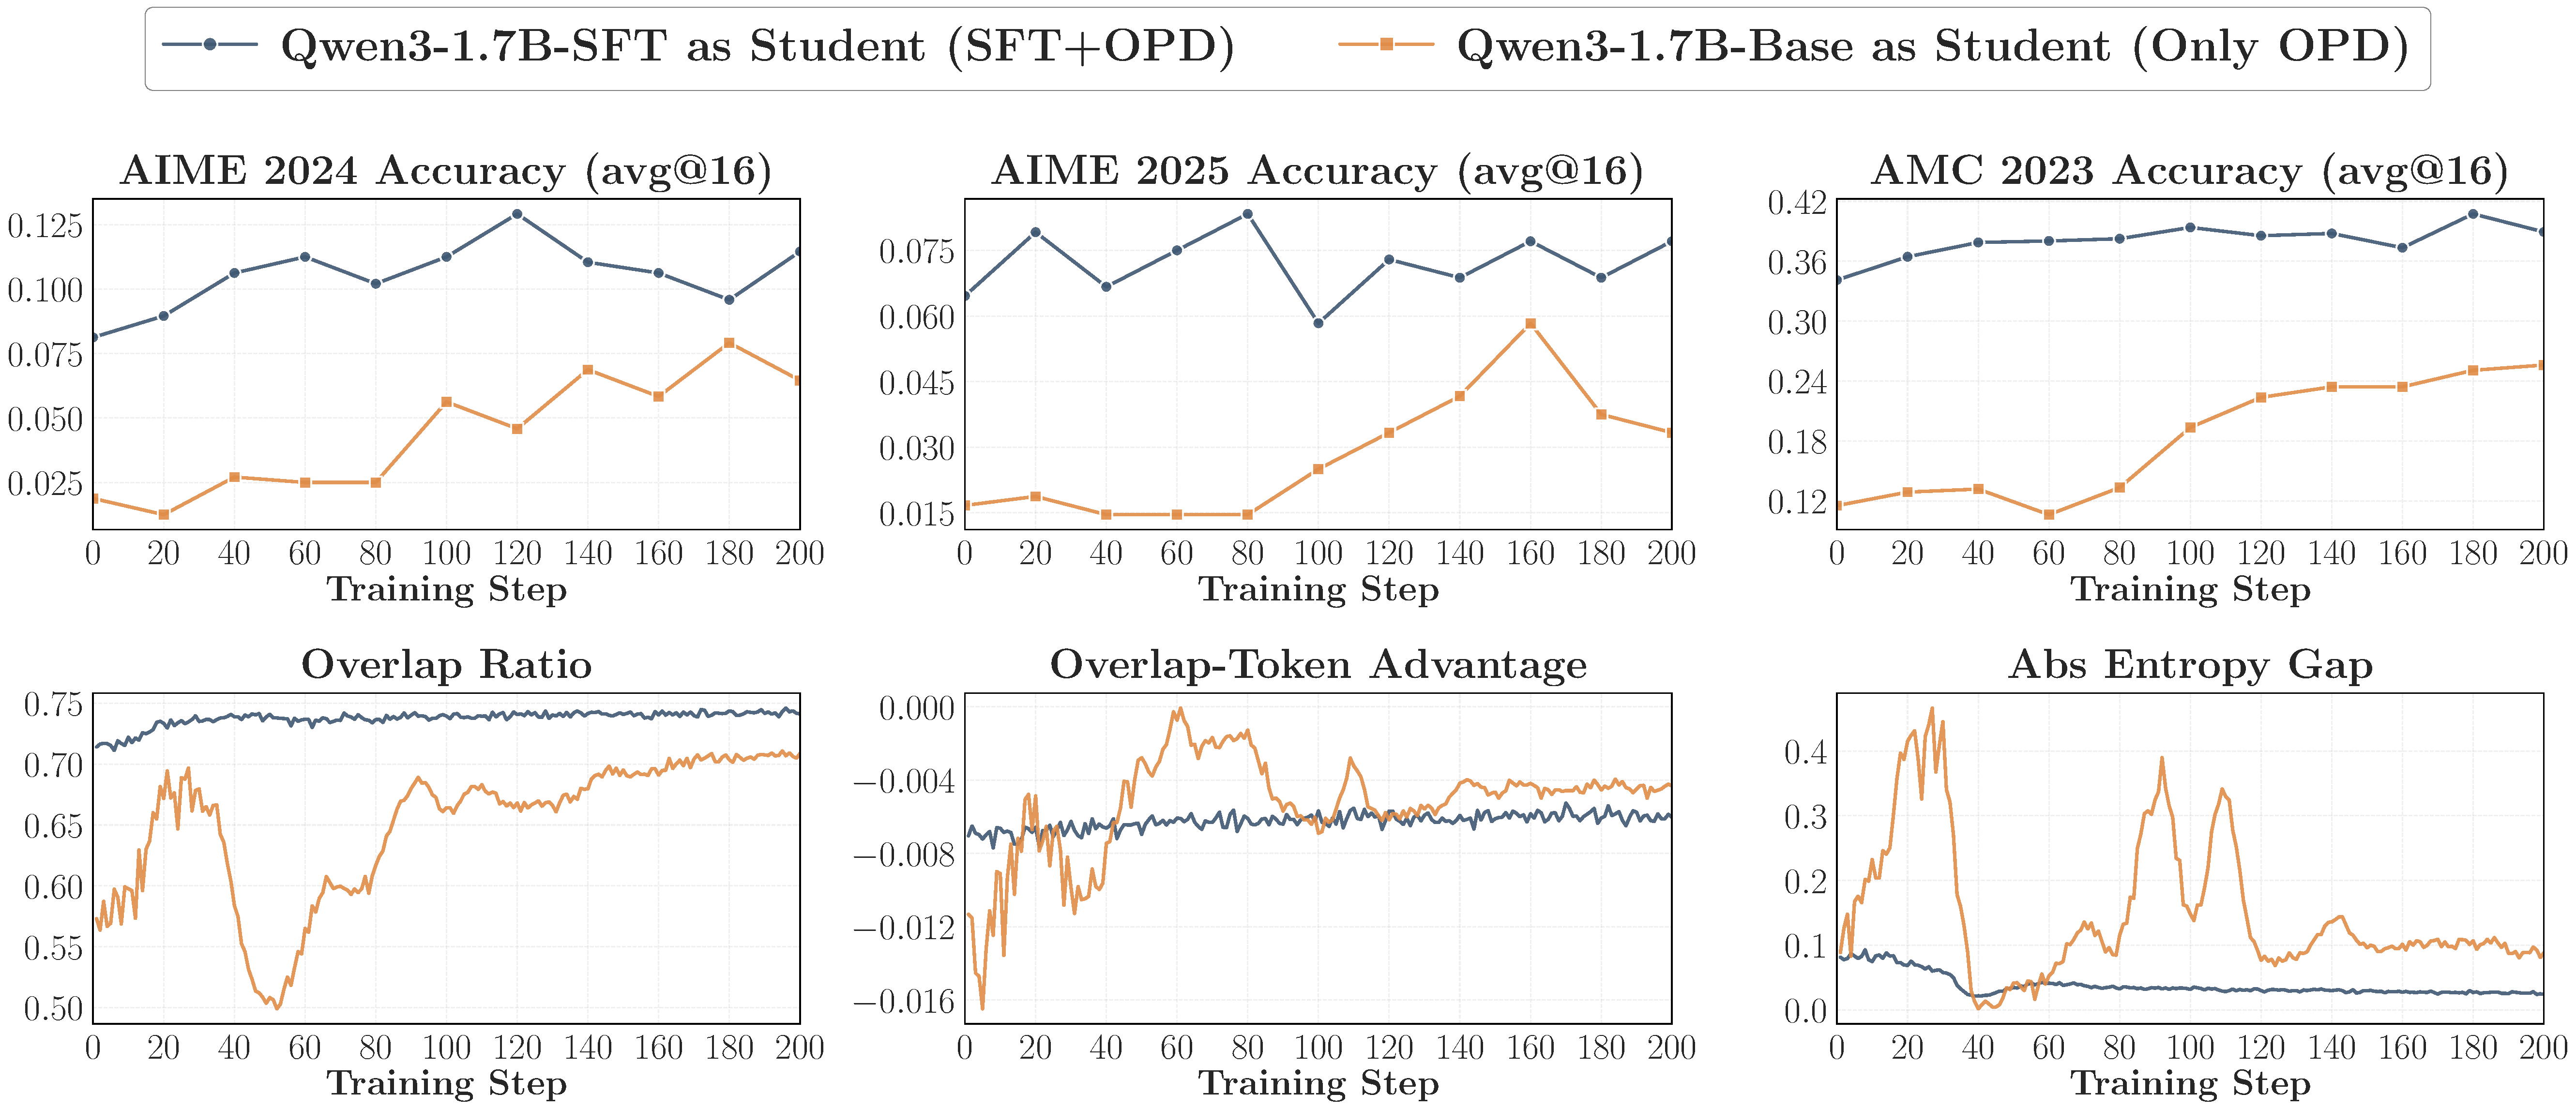
\includegraphics[width=\textwidth]{Figures/4.2/4_2_combined.pdf}
    \caption{
    Effect of off-policy cold start before OPD, using fixed teacher Qwen3-4B (Non-thinking). The two curves correspond to OPD from Qwen3-1.7B-SFT and Qwen3-1.7B-Base.
    }
    \label{fig:off_policy_distillation}
\end{figure*}


\paragraph{Setup.}
We study this setting using Qwen3-1.7B-Base as the student and Qwen3-4B (Non-thinking) as the teacher.
We use the math-domain subset of OpenThoughts3-1.2M~\citep{guha2025openthoughts} as the prompt source for SFT.
The teacher generates 200K responses on a subset of this dataset, and we use these teacher rollouts to perform SFT on the student as a cold start, yielding Qwen3-1.7B-SFT.
We then continue training with OPD from this SFT initialization, using the remaining prompts from OpenThoughts after deduplicating against the SFT prompt subset (approximately 30K prompts).
As a control, we compare against a pure-OPD baseline that starts directly from Qwen3-1.7B-Base and uses the same teacher and OPD prompt set, but performs no cold-start distillation before OPD.
Detailed offline rollout and SFT configurations are provided in Appendix~\ref{app:coldstart_details}.


\paragraph{Results.}


As shown in \Cref{fig:off_policy_distillation}, the two-stage approach substantially outperforms pure OPD. Starting from Qwen3-1.7B-SFT yields consistently better validation performance than starting directly from Qwen3-1.7B-Base. Moreover, the performance gap persists throughout training, indicating that the off-policy cold start improves not only early optimization, but also the final performance ceiling of subsequent OPD.

The overlap dynamics support the same conclusion. The SFT-initialized student begins with a much higher overlap ratio and maintains a smooth, stable trajectory, whereas the base-initialized student starts lower and exhibits pronounced instability before gradually recovering.
The entropy gap is also substantially smaller for the SFT-initialized student, indicating a closer match to the teacher's confidence profile from the outset.
These observations confirm that off-policy distillation reduces the initial pattern mismatch, making the teacher's token-level supervision immediately exploitable once OPD begins.
A more detailed analysis of the overlap mass dynamics is provided in Appendix~\ref{app:add_analysis_of_overlap_mass}.





\subsection{Leveraging Teacher Post-Training Prompts}
\label{sec:teacher_posttrain_data}

The previous section narrows the thinking-pattern gap by moving the student closer to the teacher through SFT.
Another way to improve alignment is from the data side.
Since the teacher's policy is shaped by the prompts seen during post-training, we find that using teacher-aligned prompts during OPD yields more effective supervision.

\begin{figure*}[t]
    \centering
    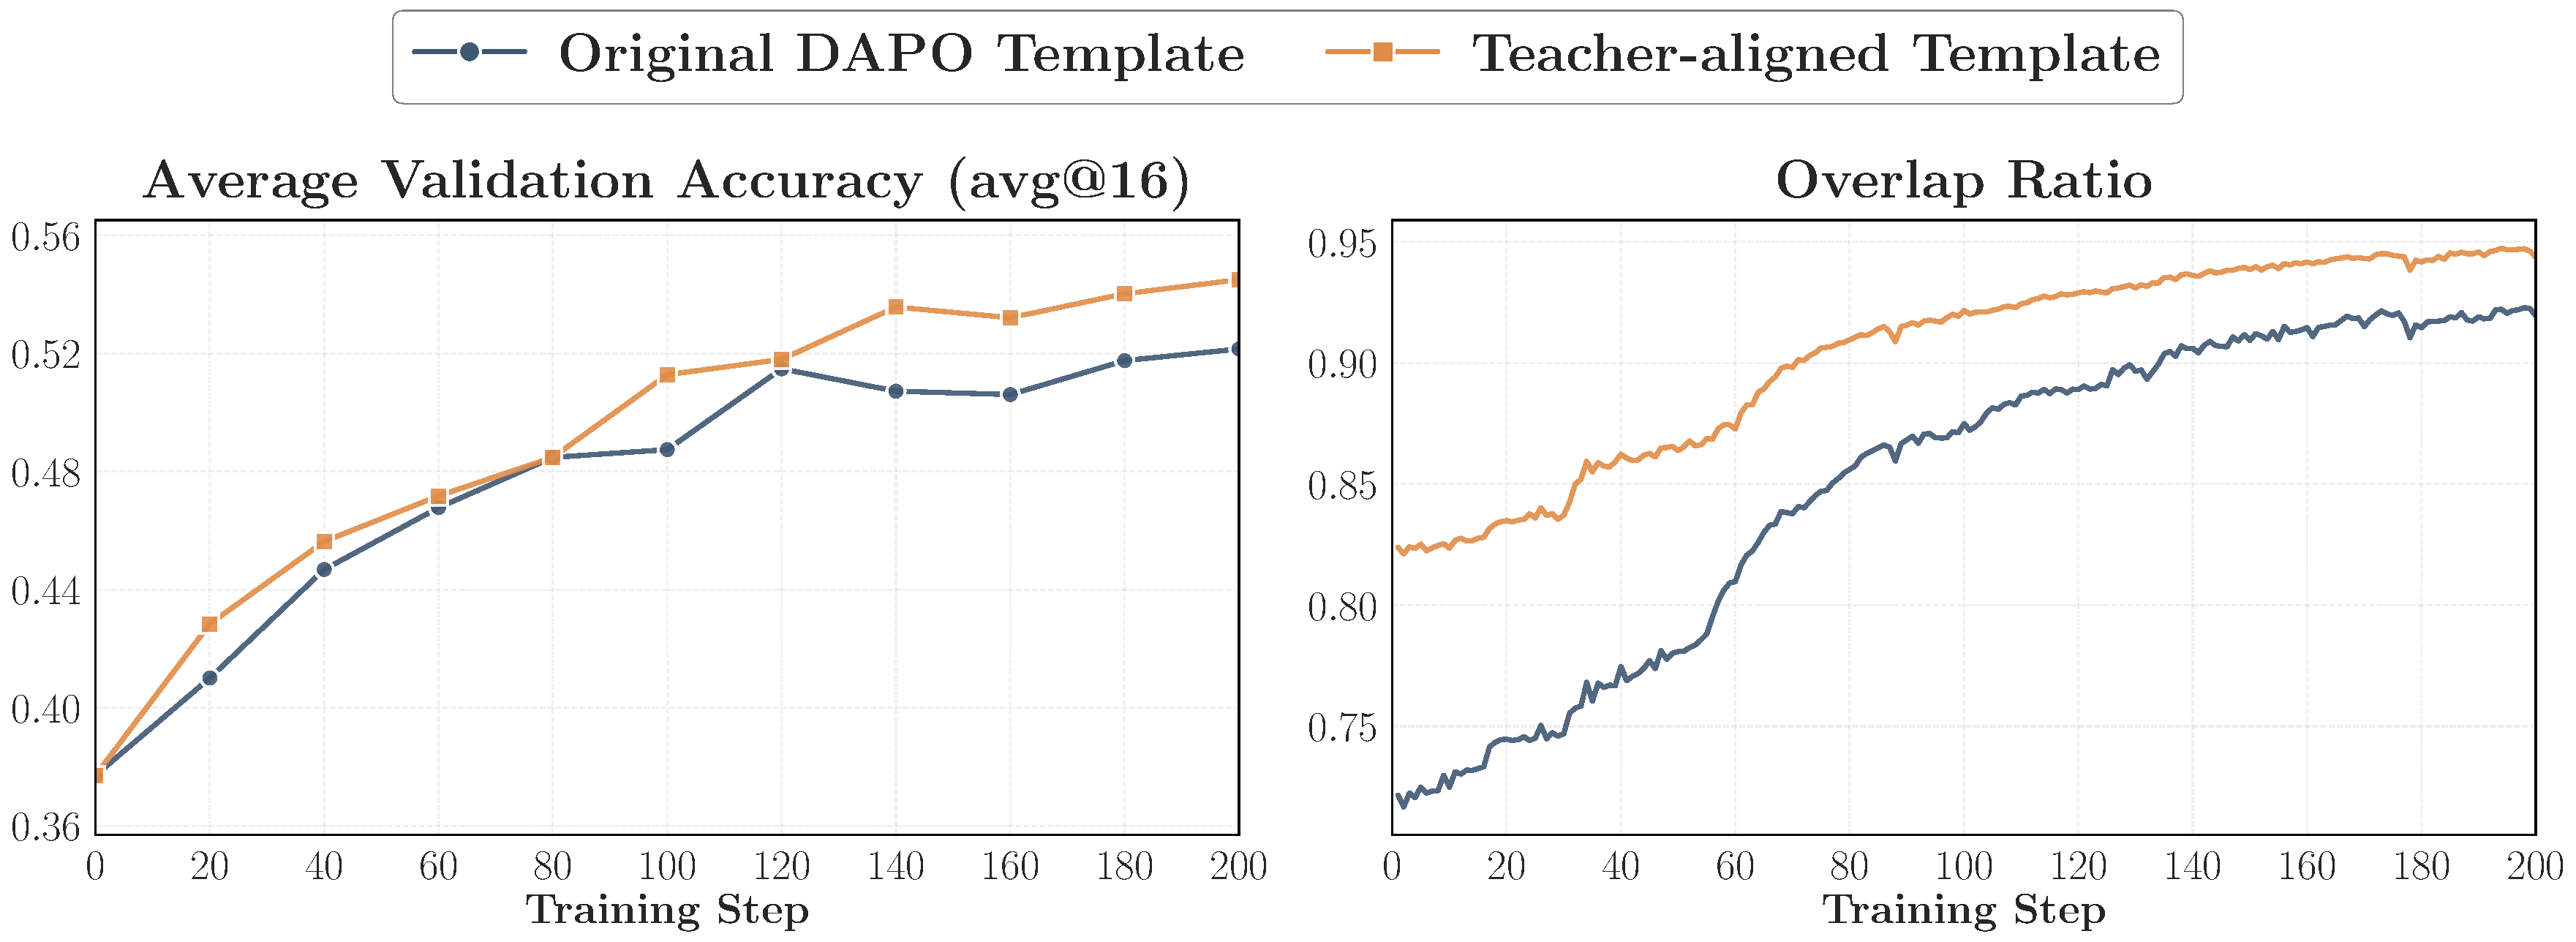
\includegraphics[width=.95\textwidth]{Figures/4.3/4_3_Same.pdf}
    \caption{
    Effect of prompt template alignment. The teacher-aligned template yields higher accuracy and overlap growth throughout training.
    }
    \label{fig:teacher_posttrain_data_same}
\end{figure*}

\begin{figure*}[t]
    \centering
    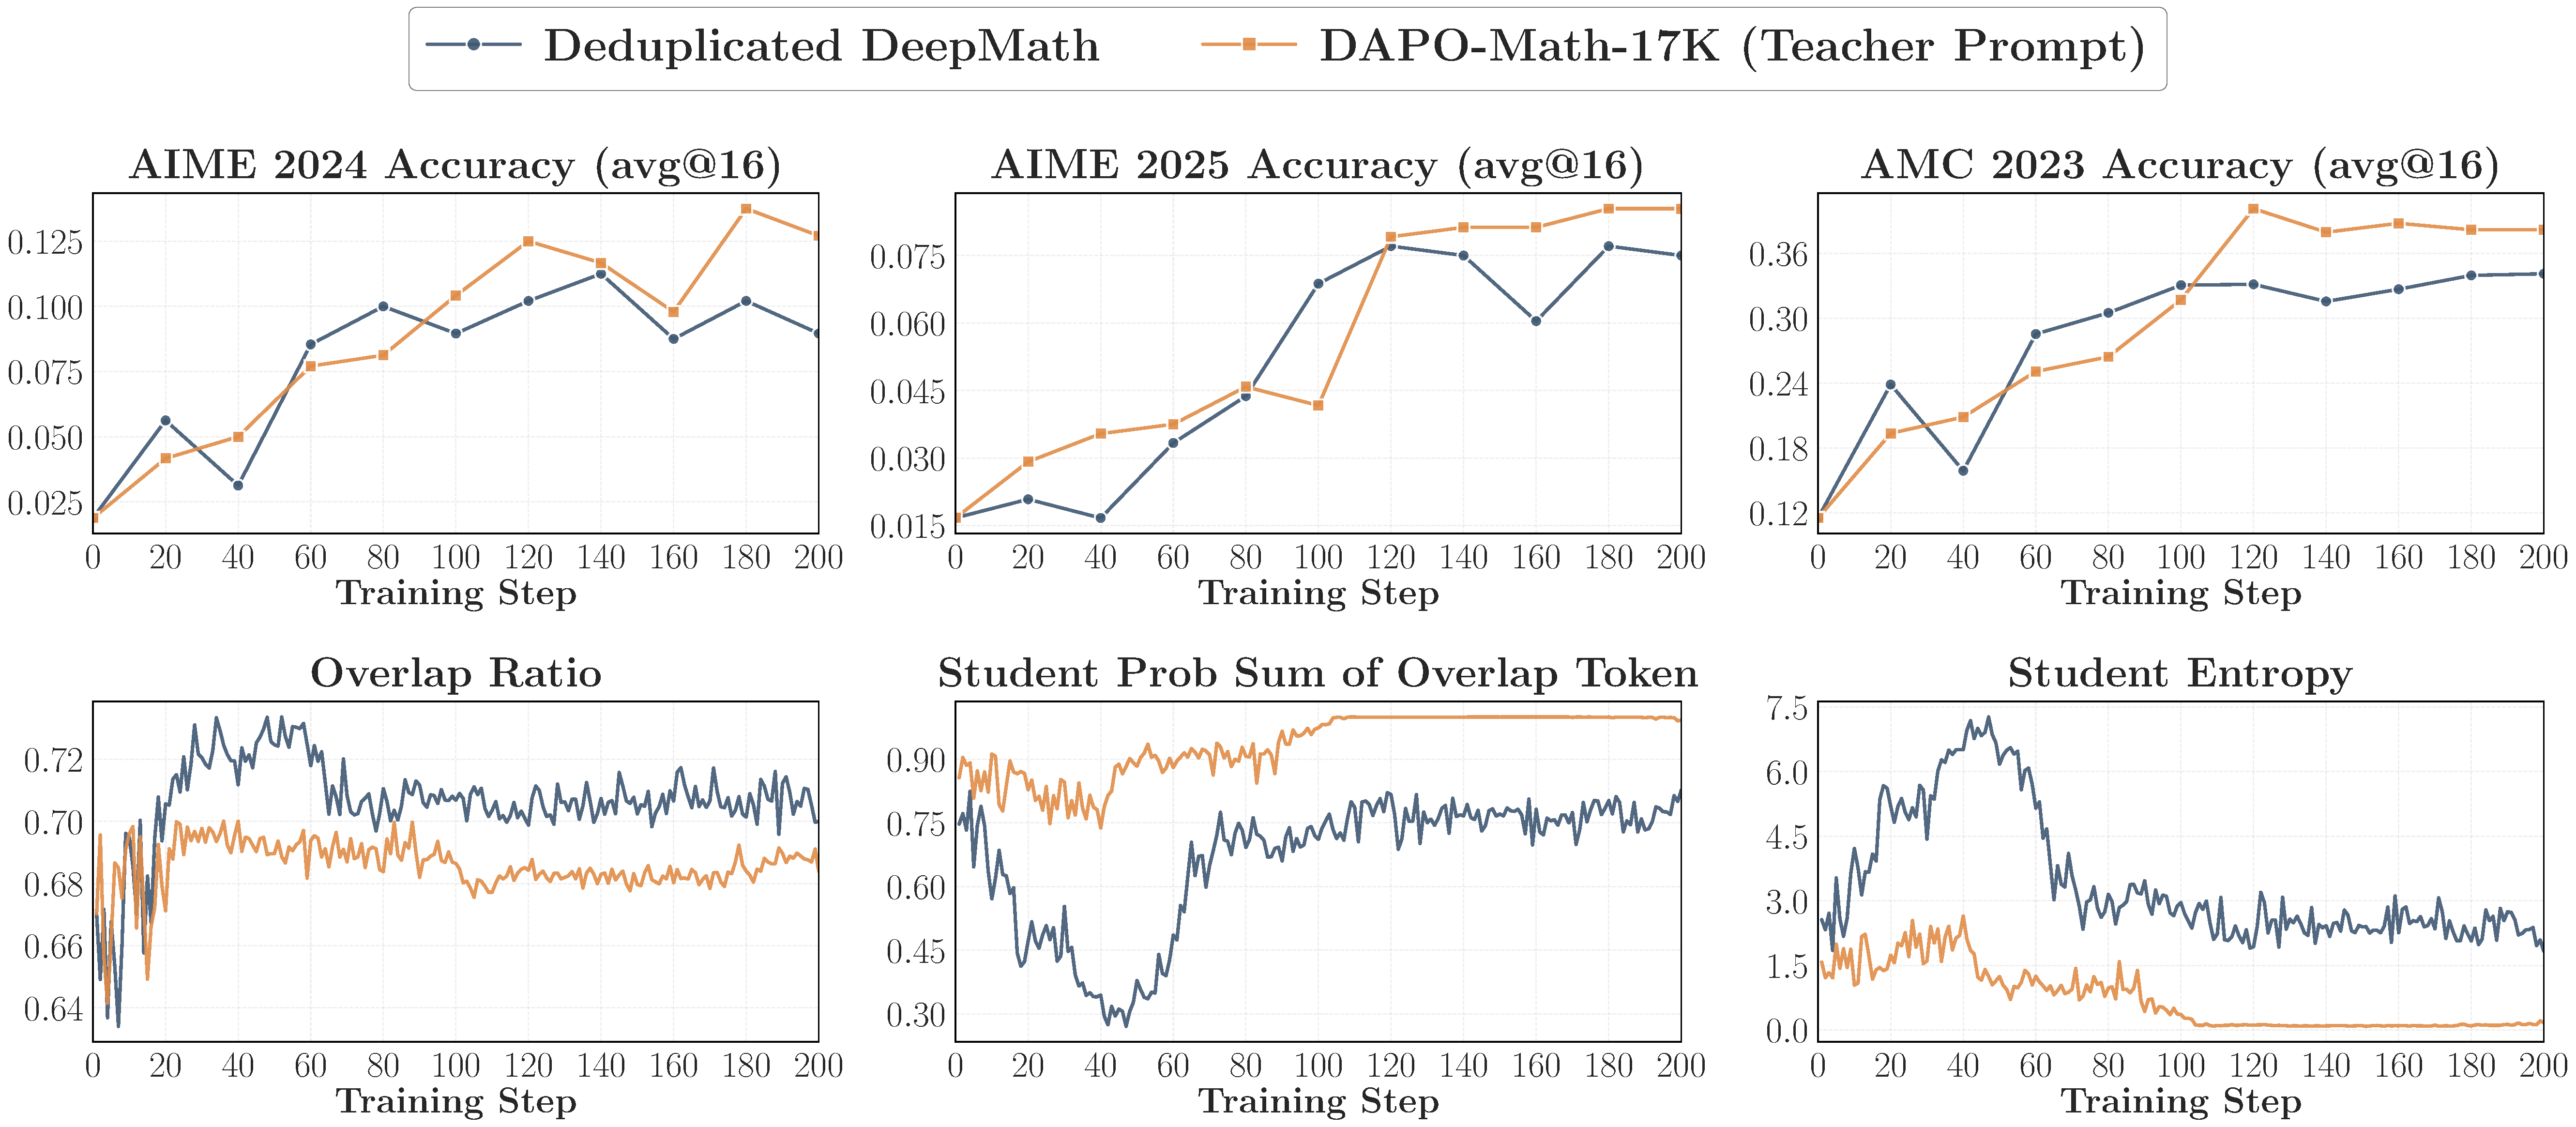
\includegraphics[width=\textwidth]{Figures/4.3/4_3_Diff.pdf}
    \caption{
    Effect of prompt content alignment. The teacher-aligned prompt contents yield stronger performance, with higher mass concentration on shared tokens and notably lower entropy.
    }
    \label{fig:teacher_posttrain_data_cross}
\end{figure*}

\paragraph{Setup.}


We conduct experiments at two granularities: whether matching the prompt \emph{template} matters, and whether matching the prompt \emph{content} matters.

\begin{itemize}[leftmargin=12pt]
    \item \textbf{Prompt template:} The teacher is JustRL-1.5B and the student is R1-Distill-1.5B. The prompt set is DAPO-Math-17K, with only the prompt template differing. The \emph{original} template is the standard DAPO format used in all previous experiments unless otherwise specified, while the \emph{teacher-aligned} template matches the format used during JustRL post-training:

\begin{tcolorbox}[title=\textbf{Original DAPO Template},colback=Salmon!20, colframe=Salmon!90!Black]
\small
Solve the following math problem step by step. The last line of your response should be of the form Answer: \$Answer (without quotes) where \$Answer is the answer to the problem. \{Question\} Remember to put your answer on its own line after ``Answer:''.
\end{tcolorbox}

\begin{tcolorbox}[title=\textbf{Teacher-Aligned Template}, colback=CornflowerBlue!20, colframe=CornflowerBlue!90!Black]
\small
\{Question\} Please reason step by step, and put your final answer within \textbackslash boxed\{\}.
\end{tcolorbox}

    Thus, the two runs contain the same math problems but differ in how the task is presented to the model. This design isolates the effect of prompt-template alignment with the teacher while keeping the underlying problem content unchanged.

    \item \textbf{Prompt content:} The teacher is Qwen3-4B-Base-GRPO introduced in \Cref{sec:thinking_pattern_consistency} and the student is Qwen3-1.7B-Base. We compare two prompt sets of matched size: DAPO-Math-17K (aligned with the teacher's RL training datasets) and a subset of DeepMath, deduplicated against DAPO-Math-17K (see Appendix~\ref{app:deepmath_dedup}). This design tests whether OPD benefits from using prompts that are identical to the teacher's post-training data, rather than prompts that are merely in-domain.
\end{itemize}





\paragraph{Results.}

The prompt template setting in \Cref{fig:teacher_posttrain_data_same} shows that simply switching to the teacher-aligned template improves validation performance on all three benchmarks.
The overlap dynamics support this result: the teacher-aligned template run begins with a higher overlap ratio and converges to a higher level, which indicates that even a minor change in prompt template can materially affect OPD by making the student's generated states more compatible with the teacher.
The benchmark-wise breakdown in Appendix~\ref{app:teacher_template_breakdown} shows the same trend.


The prompt content setting in \Cref{fig:teacher_posttrain_data_cross} shows a similar downstream advantage but with a subtlety: teacher-aligned prompts produce a lower overlap ratio throughout training. However, the cumulative student probability mass on the overlap tokens is substantially higher, indicating that the student concentrates its mass on fewer but more strongly shared tokens.
The effective alignment on high-probability tokens is therefore stronger, even though the overlap set is smaller.




\textbf{At the same time, we observe that using teacher-aligned prompts leads to substantially lower student entropy during training.}
This suggests that performing OPD only on prompts seen during teacher post-training may not always be ideal, as it can overly reduce policy entropy.
In practice, a more robust strategy may be to mix teacher-aligned prompts with prompts outside the teacher’s post-training data in order to preserve policy entropy and maintain the student’s capacity for exploration.

Overall, these results suggest that OPD benefits not only from an appropriate teacher, but also from a well-matched prompt set. Prompts closer to the teacher's post-training data can improve downstream performance and sharpen alignment on the most important shared tokens, but they should be used with care to avoid overly suppressing student entropy.
